\section{Architecture and rationale of EPS}
\label{sec:EPS_architecture_rationale}

\subsection{Available alternatives}
\label{subsec:available_alternatives}

The endeavour that Juno faces to generate enough electricity to sustain science operations at approximately 5.45 AU required particular attention in designing an efficient and reliable electric control system. Particularly, different options were present to generate the amount of power required, each of them with advantages and disadvantages:

\begin{itemize}
    \item \textbf{RTG:} the choice of a radioisotope to generate electricity could be considered. In order to generate the amount of power required around Jupiter, during the planetary phase 
    (\mref), 
    one RTG of the same size of the one present on board New Horizons spacecraft  would have been sufficient ( $\approx$ 250 We of production at BOL)\cite{nh_rtg}. Electric power requirement would also be lower as some heat could have been routed to the propulsion section to heat up the tanks and fuel lines. This choice however had some problems, mainly with respect to the safety during Earth EGA, radiation contamination, heat dissipation at distances lower than 2 AU from the Sun and weight distribution. Particular problems could have rose as the said RTG generates around 4.4 kW of heat, requiring a very efficient dissipation system for the first years of the mission, oversizing it with respect to the nominal orbit around Jupiter. Availability of Plutonium-238 was also critical as suppliers could not guarantee the needed amount of fuel, given the stop in the production of the said isotope during the 80s \cite{plutonium}. 
    
    \item \textbf{Solar panels:} no spacecraft equipped with solar panels has ever been tested at 5.44 AU from the Sun. This choice would have required a very large surface area, and thus precautions had to be taken into account inside the fairing during launch operations, to provide enough power for safe operations at Jupiter. A complex management system is also required in order to not discharge too much current inside the electronics during the ICs and the OC as the amount of solar flux hitting the S/C during different parts of the mission dramatically reduces. More stringent pointing requirements are also present as not having a clear view of the Sun could have led to the need of bigger and heavier batteries. 
\end{itemize}

Considering also the driving requirement of utilizing as much as possible off the shelf components, budget constraints, the limited supply of plutonium and the different possible configurations offered, solar panels were chosen. This choice led to a particular design of the satellite, where mass distribution was exploited to grant more stability throughout the different phases of the mission.  

\subsection{Components and distribution}
\label{subsec:components_and_distribution}

The flown spacecraft is fitted with 3 solar arrays and 2 Li-Ion batteries. 
\subsubsection{Solar arrays}
\label{susubsec:solar_arrays}

The arrays are mounted on the side of the main body, spaced 120° apart, and are composed by a different number of panels: A1 presents only 3 panels while A2 and A3 present 4 panels each. The total mass of the arrays is 340 kg, with a total area of 60 m$^2$ \cite{arrays_mass} and an active area of 49.77 m$^2$, composed by 18698 solar cells. 
Each cell, produced by Spectrolab, is in an ultra triple junction (UTJ) configuration, to obtain optimum packing and high performances in LILT environments like the one around Jupiter. The three layers, Ge for the bottom cell, GaAs for the middle cell and GaInP$_2$ for the top cell, are placed on top of a Germanium Kapton substrate and connected with tunnel junctions. A multi junction configuration optimizes the electromagnetic spectrum exploitation, focusing on specific wavelength bands. An anti-reflective Si coating protects the cell from the harsh environment of Jupiter. 

 Solar panels are linked one to the other and to the main body with electro-actuated hinges and the first panel of each array is supported by struts. All these elements are needed to both extend the panels soon after separation from the Centaur and to control the position of the arrays during all the operations. This is necessary to take into account the bending of the arrays during large manuevers and their thermal expansion. Moreover it is necessary to align the main inertia axis (Z-axis) with the spin axis due to the particular mass distribution of the panels and of the instrumentation.



Power produced by each panel is varying in each phase, depending on incidence and distance from the Sun. Fixing the attitude of the spacecraft, as the distance increases, and thus the solar flux decreases, a lower current is produced at the same voltage. However with the increase of distance, and thus the decrease of the temperature, the current decreases, the cells' efficiency increases and an higher voltage is produced. Cell efficiency at 28°C is 28.4\%.  Given that Juno's trajectory ranges between 0.88 AU and 5.45 AU from the Sun, the cells are grouped in strings of three different lengths, whose connection must be adjustable to satisfy power, voltage and current requirements in each phase. When not in use, the power generated by each cell is left on the panels to be dissipated as heat. This is crucial to ensure a high level of efficiency, increasing as temperature decreases, throughout the whole journey. 

The rationale for the distribution of the cells in each panel is shown in \autoref{fig:Solar panels reasoning.pdf} and explained as follows. 

\cfig{Solar panels reasoning.pdf}{0.7}{Cell distribution rationale}

 Once fixed the cell type used for the whole mission and known the power, voltage and current required in each phase, exploiting the characteristic curve of each cell, the number of cells that must be connected in series and in parallel can be obtained and so the required string length type. Then, as the cells' dimension is known and the length of the required strings has been retrieved, the area of each string can be computed. The mass of the panels needs to be distributed so that the inertia matrix becomes as diagonal as possible, with the constraint that only one string type can be fitted in each panel. Indeed in the case of a panel composed by all three types of strings, hot spots due to the activation of only a single type of string could lead to uneven internal stresses and thus damaging the whole panel. Moreover, damages to a single panel in this case would lead to the loss of multiple types of strings, reducing the available power during different phases of the mission. 
 
 However, given all the aforementioned requirements and considering also the limited amount of space inside the Atlas V's fairing, A3P1 had to feature both medium and short strings. The resulting string configuration is reported in \autoref{table:strings_description}. The maximum number of strings in parallel and the minimum activation distance are limits that ensure the survivability and correct operation of the system: exceeding these limits, and thus generating a current above 7A, would blow a fuse, compromising the whole mission.

 \begin{table}[H]
    \renewcommand{\arraystretch}{1.3}
    \centering
\begin{tabular}{|c|c|c|c|c|}
    \hline
    \textbf{String type} & \textbf{\# cells in series per string} & \textbf{\# strings} & \textbf{Max \# strings in parallel} & \textbf{Minimum distance [AU]}\\
    \hline
    \hline
    \textbf{Long}    &  22 & 114 & - & 0.88 \\
    \hline
    \textbf{Medium}  &  14 & 369 & 40 & 1.8\\
    \hline
    \textbf{Short}   &  13 & 848 & 64 & 3.8 \\
    \hline
\end{tabular}
\caption{Strings description}
\label{table:strings_description}
\end{table}

Consequently, as can be seen in \autoref{table:panels_area} and \autoref{table:panels_mass}, A2P1, A2P2 and A2P3, and the same in A3, are slightly smaller than the A1 correspondents while the presence of A2P4 and A3P4 counterbalances the presence of the MAG boom on the tip of A1. 

\begin{minipage}{0.45\linewidth}
    \centering
    \captionsetup{type=figure}
    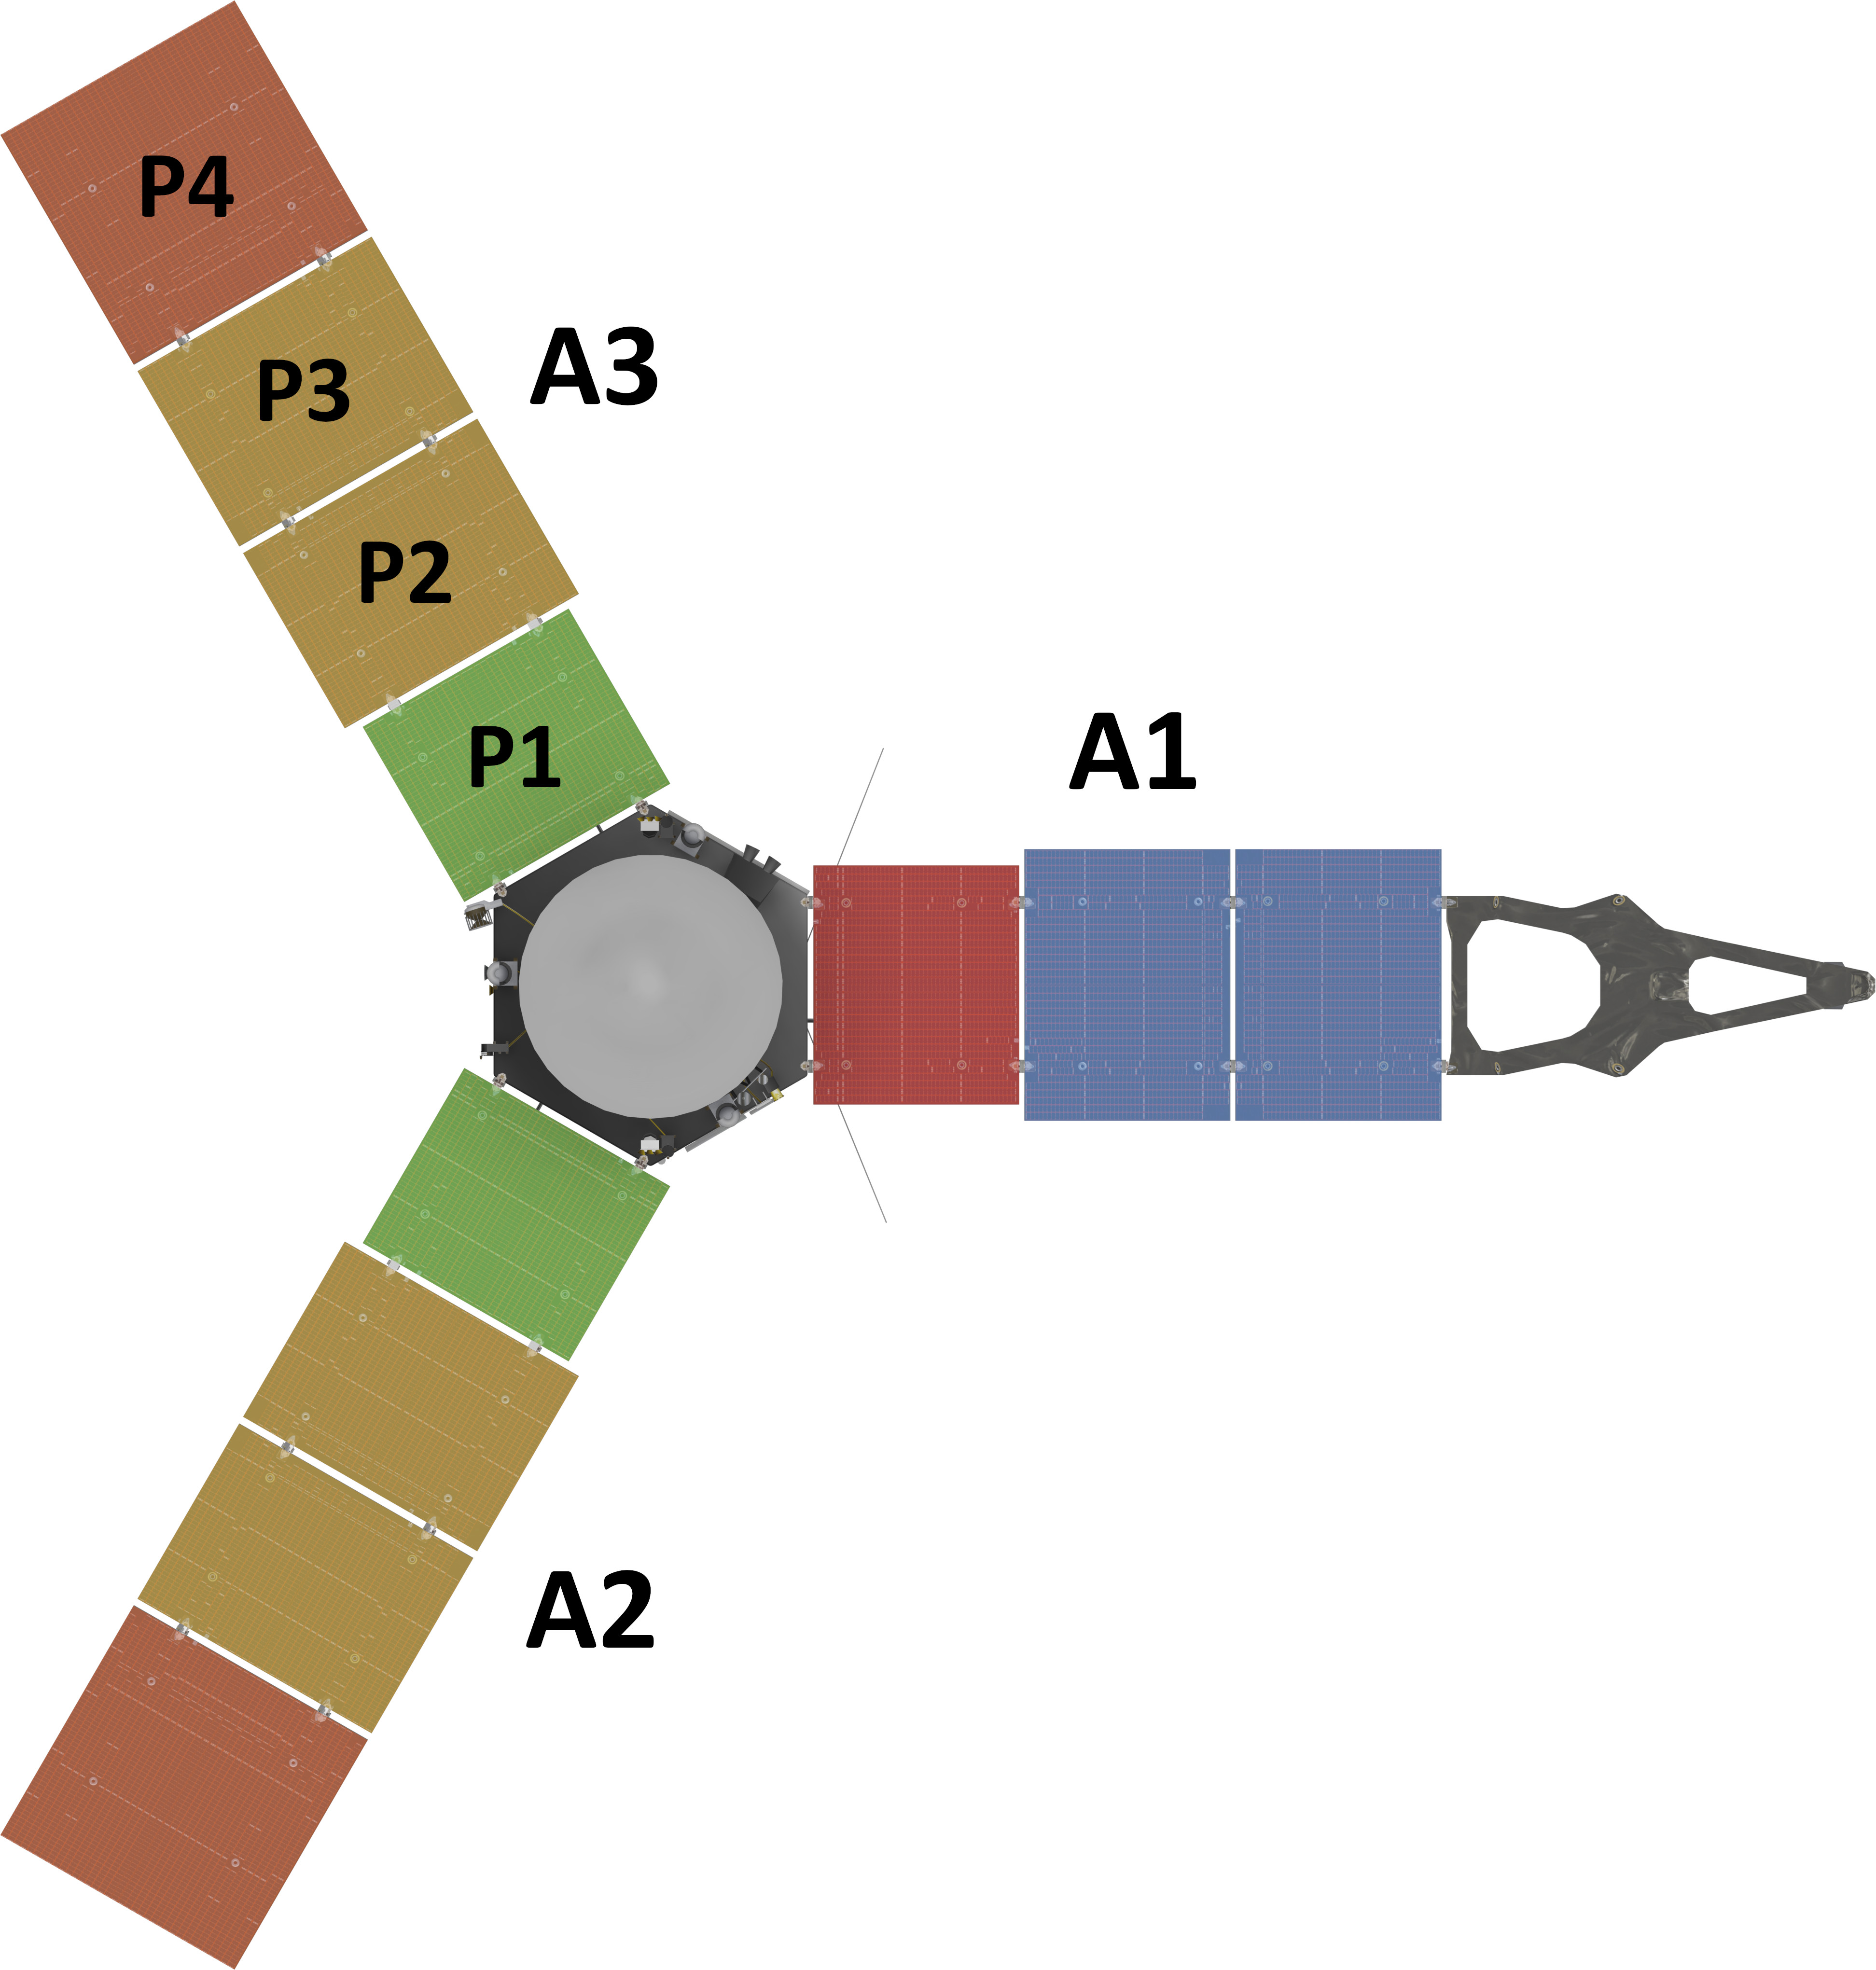
\includegraphics[width=\linewidth]{Images/Juno panels.jpg}
    \caption{Juno's panel configuration}
    \label{fig:panel_config}
\end{minipage}\hfill
\begin{minipage}{0.5\linewidth}
    \centering
    \captionsetup{type=table}
    \renewcommand{\arraystretch}{1.4}
    \begin{tabular}{|c|c|c|c|c|c|}
        \hline
        &  \textbf{P1}  & \textbf{P2} & \textbf{P3} & \textbf{P4} & \textbf{Array's area} \\
        \hline
        \hline
        \textbf{A1}      & 4.92 & 5.60 & 5.60 & - & 16.11  \\
        \hline
        \textbf{A2}      & 4.81 & 5.46 & 5.46 & 6.29 & 22.02 \\
        \hline
        \textbf{A3}     & 4.81 & 5.46 & 5.46 & 6.29 &  22.02 \\
        \hline
    \end{tabular}
    \caption{Panels areas [m$^2$]}
    \label{table:panels_area}

    \vspace*{3mm}

    \begin{tabular}{|c|c|c|c|c|c|}
        \hline
        &  \textbf{P1}  & \textbf{P2} & \textbf{P3} & \textbf{P4} & \textbf{Array's mass}\\
        \hline
        \hline
        \textbf{A1}      & 27.81 & 31.62 & 31.62& - & 91.05 \\
        \hline
        \textbf{A2}      & 27.17 & 30.89 & 30.89 & 35.54 & 124.47 \\
        \hline
        \textbf{A3}     & 27.17 & 30.89 & 30.89 & 35.54 & 124.47 \\
        \hline
    \end{tabular}
    \caption{Panels masses [kg]}
    \label{table:panels_mass}
\end{minipage}

% !! nella batteria mettere voltaggio

\subsubsection{Batteries}
\label{subsubsec:Batteries}
Juno is equipped with two Li-Ion batteries in cold redundance: these ensures complete operability throughout thw whole mission, even 

% due per ridondanza, qualche caratteristica dal datasheet. 
% dove sono
% a cosa servono
% livello scarica e cicli 